
\chapter{Metodologia}

Para o estudo, foi realizada uma pesquisa qualitativa através de entrevistas semi-estruturadas utilizando como base a entrevista desenvolvida pelo artigo base \cite{empiricalStudy2016}. A primeira seção abordará uma visão geral sobre os primeiros passos da pesquisa.  Já a segunda seção discorre sobre como as entrevistas foram conduzidas. Na terceira, encontra-se todo o processo utilizado para a análise dos dados obtidos na entrevista. Por último, a quarta seção mostra informações a respeito dos participantes da pesquisa.


\section{Pré-estudo}

Com o objetivo de entender melhor sobre como as práticas de CI/CD migraram para as empresas sediadas em Recife, dois pesquisadores realizaram um pré-estudo. Primeiramente, foi discutido a respeito do artigo base \cite{empiricalStudy2016}. Na discussão foi definido que seria replicado apenas o estudo baseado em entrevistas semi-estruturadas para garantir o entendimento dos termos pelos entrevistados e a adequação com as definições do artigo base. 

Após a discussão, os entrevistadores acessaram o apêndice online deste \cite{empiricalStudyOnlineAppendix} para obter o guia de entrevista utilizado. Como forma de manter a consistência, foi utilizado o mesmo guia de entrevistas, assim como as mesmas definições utilizadas pelos autores. No início foi montado um arquivo com a definição de cada um dos termos envolvidos em língua portuguesa para ser utilizado como consulta caso haja alguma dúvida de definição de tópicos entre os entrevistadores.

Após isso, o guia de entrevistas do estudo base \cite{empiricalStudyOnlineAppendix} também foi traduzido para português e utilizado durante as entrevistas. Um ponto importante a respeito da tradução é o fato de que alguns termos ainda foram mantidos na língua inglesa devido ao fato de serem conhecidos mundialmente nesta língua. Por exemplo, Continuous Integration, Canary Releases e Health check.
O documento de consulta e a guia de entrevistas estão presentes no apêndice deste trabalho, ambos em sua versão traduzida.

\section{Estrutura da Entrevista}

O guia de entrevistas se baseia na estratégia de evitar perguntas diretas (exemplo: “determinada prática está sendo utilizada?”). Esse modelo é essencial para garantir que a comparação entre participantes a respeito do uso ou não de práticas está sendo feita de maneira concisa, e não baseada nos conhecimentos prévios de cada participante. Assim, através de perguntas sobre o processo utilizado pelo entrevistado é possível, com uma certa margem de erro associada, afirmar que práticas ele utiliza. A margem de erro surge do fato de o autor ter que refletir sobre as informações recebidas e as definições para inferir o uso ou não de certa prática.

A entrevista é dividida em 5 sessões: 

\begin{enumerate}
\item Processo de entrega no geral
\item Papéis/Responsabilidades
\item Garantia da Qualidade (Quality Assurance)
\item Gerenciamentos de Problemas
\item Avaliação de Entrega
\end{enumerate}

No guia, todas as sessões iniciam com uma questão aberta. As entrevistas seguiram os tópicos abordados em cada uma delas, mas sem ordem específica, respeitando o desenrolar da conversa. A primeira entrevista foi guiada pelos dois pesquisadores para assegurar que as próximas seriam feitas de forma semelhante pelos dois. Esta entrevista foi considerada como válida na análise de dados visto que não houve nenhuma mudança no questionário de entrevistas; o próprio já tinha sido validado no artigo utilizado de base para este trabalho. As outras 10 - totalizando 11 entrevistas feitas - foram guiadas por apenas um entrevistador, sendo 5 feitas por cada um dos dois pesquisadores.


Todas as entrevistas ocorreram de forma online, através do Google Meet, e aconteceram entre os meses de Setembro e Outubro de 2020 em português brasileiro. As entrevistas levaram entre 30 e 65 minutos, duração bem parecida com os tempos obtidos no artigo base (35 a 60 minutos), totalizando 7 horas e 15 minutos. Cada uma delas foi gravada pela plataforma para futura análise e 4 delas foram transcritas para o uso em citações neste trabalho, escolhidas através da relevância da entrevista e da forma como certos termos e processos foram apresentados pelo entrevistado. Foi deixado claro em cada uma das conversas a respeito da gravação e que estas seriam utilizadas apenas pelos entrevistadores, respeitando assim o anonimato de informações pessoais como nome ou empresa da qual o profissional se referia.

\section{Análise dos Dados}

\begin{figure}[ht]
\begin{center}
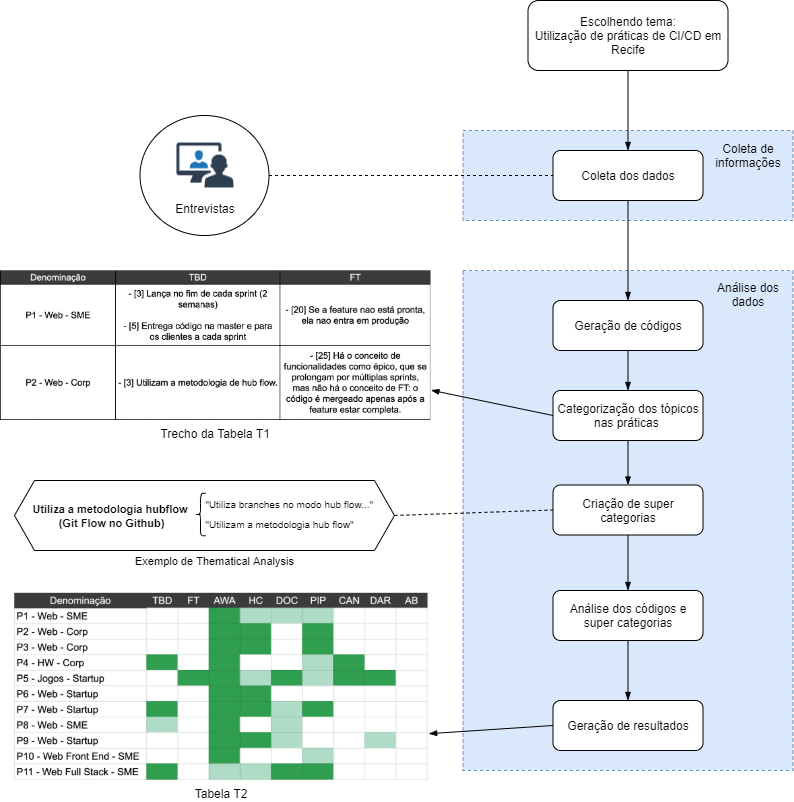
\includegraphics[scale=0.5]{metodologia_tcc.png}
\end{center}
\caption[Fluxograma da Metodologia]{
    Demonstra como funcionou o processo de coleta e análise de dados.
}\label{fluxograma_metodologia}
\end{figure}

    
A \figref{fluxograma_metodologia} apresenta uma visão geral de como funcionou o processo de coleta e análise de dados. A análise foi feita apenas pelo autor deste artigo. O processo escolhido foi baseado nas fases de \emph{Coding} e \emph{Thematic Analysis} da metodologia \emph{Grounded Theory} \cite{groundedTheory}. No processo de Coding a ideia é levantar rótulos ou tags relevantes para o texto e, tradicionalmente, é feito baseado na transcrição das entrevistas. No entanto, neste trabalho o autor gerou códigos através da escuta das entrevistas. Então, como um exemplo, a seguinte citação:

\begin{quotation}[]{P5}
"Como somos uma equipe muito pequena, todos os desenvolvedores são meio que DEVOPS. Quando tem que tomar alguma decisão nós entramos em discussão e definimos por nós."
\end{quotation}

Gerou o código: \emph{"Todos os desenvolvedores são devops."} - P5\_15

É importante salientar que os códigos gerados sofreram um certo enviesamento visto que este trabalho é uma replicação de um estudo, então o autor tinha em mente que assuntos estavam sendo procuradas na fala durante o levantamento de códigos. 

Então, após levantados todos os códigos de uma entrevista, estes foram revisados para garantir semântica e sintaxe adequadas. Alguns códigos nessa fase foram eliminados por redundância, enquanto outros foram quebrados em múltiplos. Depois, eles foram agrupados, quando compatíveis, em cada uma das 9 práticas descritas pelo artigo base e foi escolhida uma nota entre 0 a 2, representando não utiliza, utiliza parcialmente e utiliza completamente baseado nas definições do artigo base traduzidas. Este processo foi então replicado para cada uma das 11 entrevistas.

Ao final do processo ainda haviam 3 ligações entre a prática de \emph{Dark Launch} e entrevistados que não tinham recebido nenhum código em comum. Para estes casos, foi enviado um email diretamente para cada um dos entrevistados com a definição do artigo base da técnica e foi perguntado se o entrevistado utilizava ou não a mesma, o que gerou mais 3 códigos. Ao final, 292 códigos surgiram ao todo.

O agrupamento entre códigos e práticas gerou a Tabela T1, que mostra uma visão geral de cada relação entre prática e entrevistado, contendo a nota dada e os códigos que justificam a nota. Esta tabela contém 147 códigos.

De posse da tabela T1 foi gerada a Tabela T2, que contem uma visão reduzida da primeira, contendo apenas as notas de cada uma das práticas para cada um dos entrevistados com as colunas ordenadas de acordo com o \emph{Stairway to Heaven} descrito no artigo base. Com a Tabela T2, também foi criada uma nova Tabela T3 com o mesmo formato da primeira, mas com as colunas ordenadas pela utilização de cada prática em ordem decrescente. Esta tem como objetivo replicar a Tabela 1 do artigo base \cite{empiricalStudy2016}.

Por fim, para identificar padrões e abstrações nos códigos agrupados na Tabela T1, foi feito um trabalho de agrupamento semântico, gerando por fim a tabela T4 apresentando as novas super categorias geradas no processo de \emph{Thematic Analysis}. Neste, 17 super categorias foram geradas.

É importante salientar que ainda durante o processo de levantamento de códigos surgiram tópicos relevantes que não se relacionavam diretamente com as práticas descritas, mas que são perguntados pelo questionário e relevantes para o tema tratado. Surgiram então 2 novas colunas que agregavam códigos sobre as práticas de \emph{Code Review} e de testes automáticos. Para estas foram relacionados 29 códigos, e duas super categorias foram geradas.

\section{Participantes}

No total foram entrevistados 11 desenvolvedores (P1 a P11) de 7 empresas diferentes sediadas em Recife. Destes, 3 eram mulheres. Pode-se ver a distribuição dos participantes entre gênero na \figref{genero}. Dentro desse grupo, 9 trabalhavam com aplicações Web, enquanto 1 trabalhava com sistemas embarcados e o último, com jogos.

\begin{figure}[ht]
\begin{center}
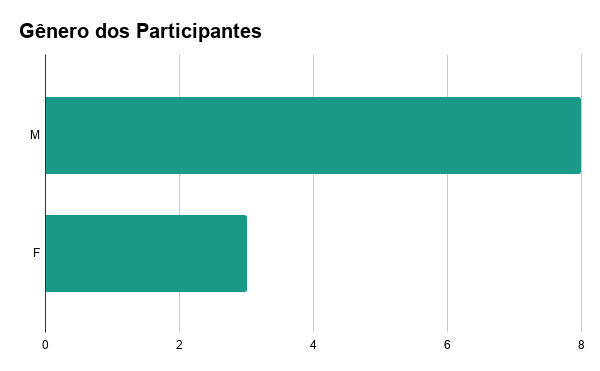
\includegraphics[scale=0.5]{demographics-genero.png}
\end{center}
\caption[Distribuição dos Participantes por gênero]{
    Distribuição dos Participantes por gênero
}\label{genero}
\end{figure}

A escolha dos entrevistados foi feita baseado na rede de conhecidos dos entrevistadores, com o propósito de agregar pessoas de que trabalhavam em empresas de tamanhos distintos para garantir uma variedade de parâmetros envolvidos. Como é possível perceber na \figref{tamanho_empresa}, com relação a esse aspecto a amostra está bem distribuída. 


\begin{figure}[ht]
\begin{center}
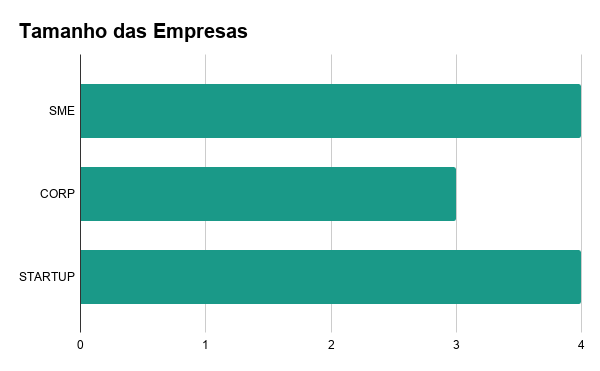
\includegraphics[scale=0.5]{demographics-tamanh-das-empresas.png}
\end{center}
\caption[Distribuição dos Participantes por tamanho da empresa]{
    Distribuição dos Participantes por tamanho da empresa.
}\label{tamanho_empresa}
\end{figure}


